

The fuel conumption and carbon pollution caused by 
driving activities are drawing more and more attentions. 
In 2013, the White House issued a climate action plan to reduce fuel consumption
and carbon pollution \cite{whitehouse2013}. 
In the same year, Morgan Stanley reported that 
there will be \$158 billion annual savings in the US 
if all cars adopted smooth driving styles \cite{morganstanley2013}. 
We introduce a driver assistance system, called EcoDrive, 
that can improve the fuel efficiency of a vehicle's drive by sensing, computing, 
and actuating the acceleration behavior of the vehicle in an autonomous manner, 
by modeling properties of the vehicle, road conditions, and driving actions. 
With the global push for improving fuel efficiency of vehicles to 
reduce consumptions and carbon emissions, 
we believe solution such as ours can be one of many important mechanisms to meet such a goal.


\begin{figure}[t]
\begin{center}
\vspace{-0.5cm}
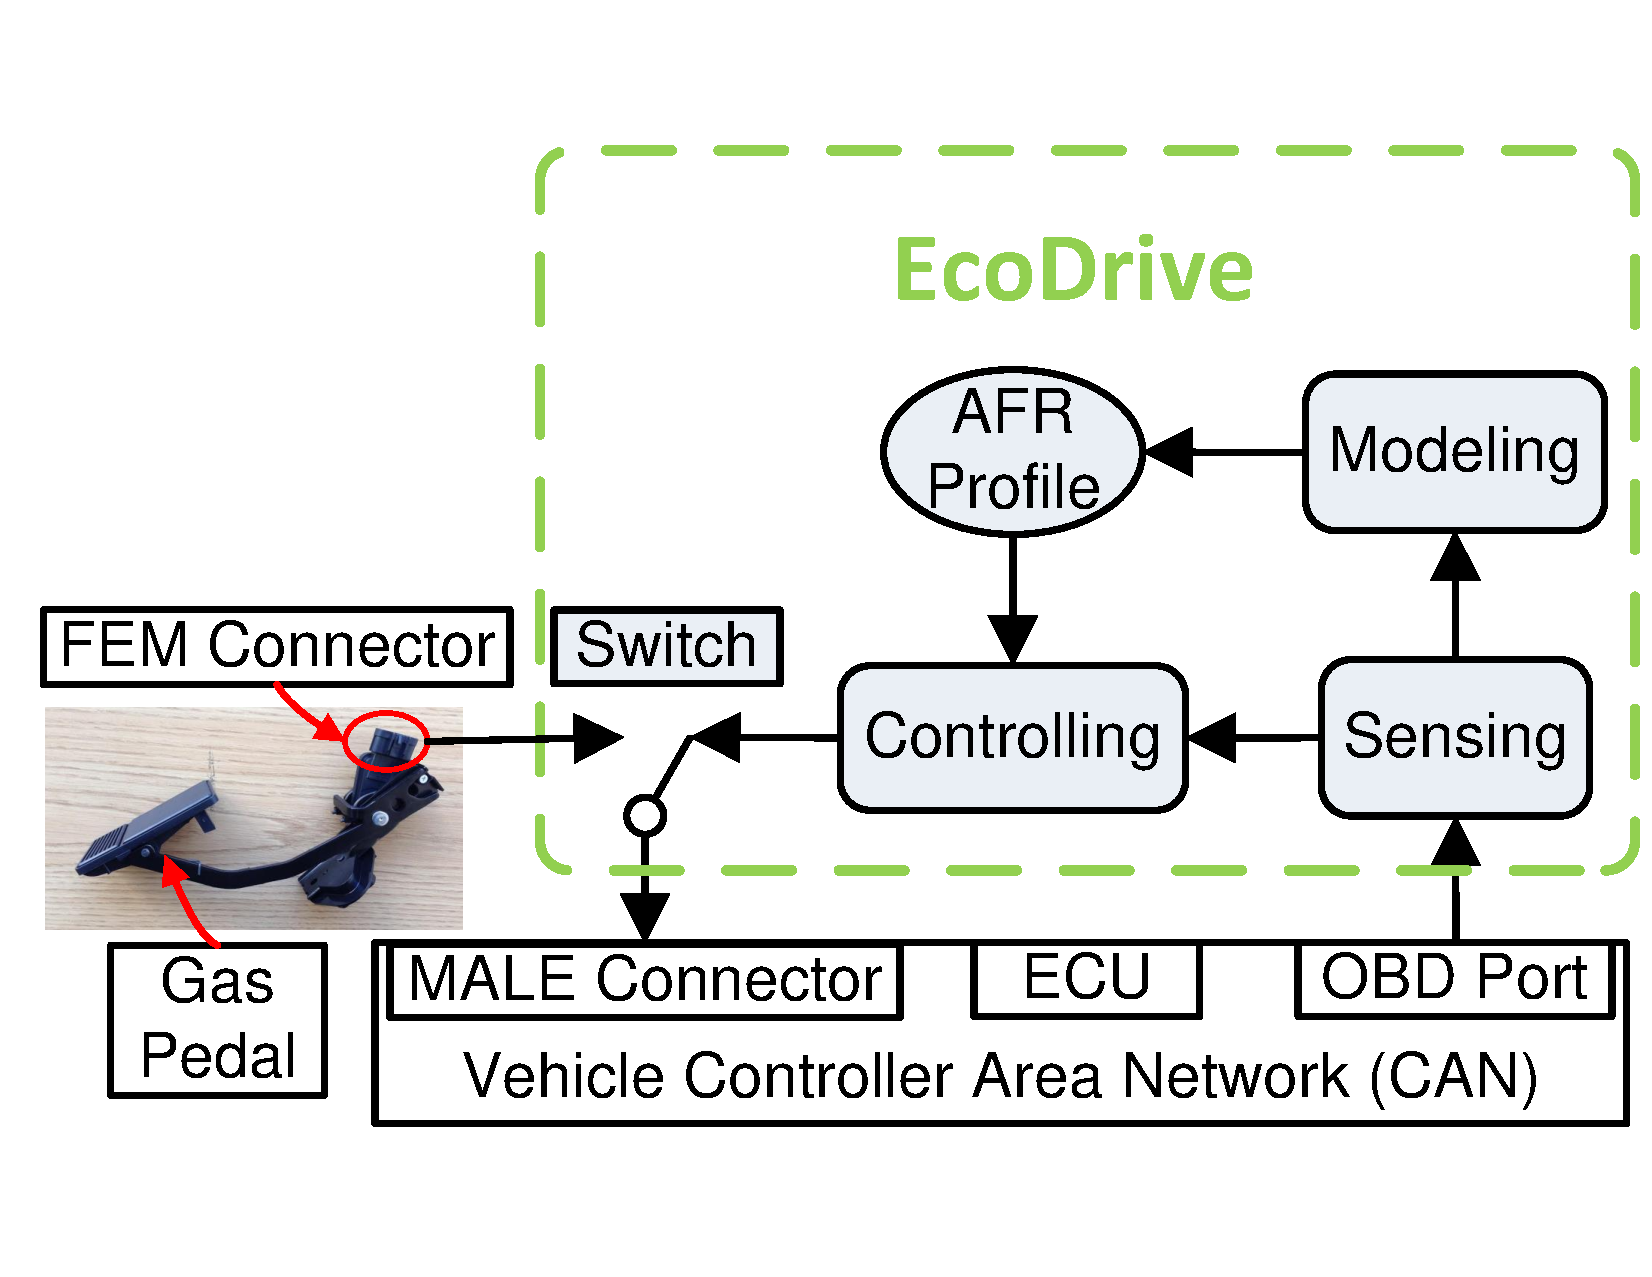
\includegraphics[width=4.0in,angle=0]{Figs/EcoDrive/architecture.pdf}
\vspace{-0.5cm}
\caption{EcoDrive Architecture.}
\vspace{-0.7cm}
\label{ecodrive}
\end{center}
\end{figure}


EcoDrive estimates instant fuel consumptions of different driving behaviors
based on sensed vehicle parameters from the On-board diagnostics (OBD) port \cite{obd, pid}. 
It can adjust vehicular speed in real time according to 
individual vehicle properties and road conditions 
to achieve higher fuel efficiency measured by Kilometer Per Liter (KPL)
\footnote{KPL refers to the distance travelled per unit volume of fuel consumed. 
It interchangeable with Mile Per Gallon (MPG), i.e., 1 KPL = 2.35214583 MPG.}.
EcoDrive is an independent system that can be installed on or removed from 
regular vehicles easily. 
This system controls the vehicle's acceleration and speed 
to provide a fuel efficient drive on its path. 
In our work and current implementation, 
we design this system assuming there is no other factors that 
would contribute to a choice of acceleration and speed, 
e.g., other vehicles, pedestrians, etc. or other obstacles in vicinity. 
Clearly in a practical system, this knowledge would be critical in modifying the acceleration behavior. 
Currently, we adopt the approach followed by other equivalent systems, 
such as cruise control \cite{cruise_control}, which allows the driver to instantly 
disable cruise control by actively pressing the brake pedal. 
In an analogous way, in our current implementation, 
we provide the driver a switch which can be pressed to instantly disable EcoDrive, 
if its acceleration behavior is perceived to be unsafe for nearby vehicles or obstacles.






\textbf{EcoDrive Components}. 
EcoDrive delivers its design via three components including an OBD sensing component, 
a vehicle dynamics modeling component and an acceleration controlling component. 
The architecture is illustrated in Fig. \ref{ecodrive}. 
The sensing component reads real-time OBD parameters through
the OBD port. 
The modeling component models various vehicle forces 
as functions of instant fuel consumption and produces
a fuel consumption profile, called Air/Fuel Rate (AFR) profile
\footnote{AFR refers to the volume of air/fuel cost per unit time.}.
The controlling component utilizes the AFR profile to calculate fuel efficient
driving strategies according to speed limit and road conditions. 
EcoDrive emulates the gas pedal by sending voltage values to 
the connector through an Arduino board.
The vehicular Electronic Control Unit (ECU) controls air/fuel injection rate
according to the voltage inputs. 

EcoDrive addresses two main challenges. 


%\textbf{How to model vehicle dynamics and build AFR profile by using OBD parameters, 
%given various vehicle types, transmission types and road conditions?}
\textbf{a) Model Vehicle Dynamics based on OBD Parameters}.
EcoDrive uses the OBD parameters delivered by
the sensing component to build an AFR profile, 
which records instant fuel consumptions of various accelerations under different speeds. 
To this end, EcoDrive models various vehicle forces, 
including propulsion, drivetrain loss, wind resistance
and grade resistance, as functions of instant fuel consumption.  
First, we model propulsion (or output torque) as a function of engine
torque and gear ratio \cite{vong2006prediction, giannelli2005heavy}. 
We use AFR to model engine torque, and use the ratio between RPM
and vehicular speed to model gear ratio. 
Second, we represent drivetrain loss and wind resistance as a function
of vehicular speed \cite{andersson2012online}.
The coefficients are estimated from recorded data traces where
the car is driving at constant speeds. 
The basic idea is that the sum of resistances is equal to
propulsion when the car is driving at a steady-state speed. 
Third, we model grade resistance by altitude changes over road segments. 
The altitudes of the locations are obtained from 
National Elevation Dataset \cite{nationalelevation}.   
Based on the three models, AFR is modeled as a function of 
speed, acceleration and road conditions. 


\textbf{b) Control Air/Fuel Rate and Vehicular Speed to Improve Fuel Efficiency}.
%\textbf{How to control accelerations and cruising speeds to improve
%gas mileage, given various road segment lengths and speed limits?}
EcoDrive controls vehicular speed by emulating gas pedal. 
It sends the emulated gas pedal position values to the
Arduino board which then converts the position
values to corresponding output voltages.
The output voltages are delivered to the ECU through a 6 Pin Connector.  
The problem is how to adjust vehicular speeds to travel through
a certain distance with the lowest fuel consumption.
We solve this problem by using dynamic programming. 
Each state of the dynamic programming model records 
the minimum air/fuel cost that allows the car to achieve
the current speed at the current location. 
In this model, speed can only increase and the last state of each
speed records the minimum fuel consumption if the car reaches the pre-assigned distance at that speed. 
We call the speed with minimum fuel consumption the target speed.  
By backtracking the state matrix from the last state
of target speed, EcoDrive can obtain the desired AFR at each speed. 
EcoDrive adjusts air/fuel injection rate based on real-time sensed vehicular speed. 
Once the vehicular speed reaches the target speed, EcoDrive
enters a cruising state and commands a constant air/fuel injection rate
until the car reaches the pre-assigned distance. 



\textbf{EcoDrive Prototype}. We build a prototype of EcoDrive in an off-the-shelf mobile embedded platform. 
The prototype is installed and tested on a 2011 Chevrolet Impala. 
We test EcoDrive on the Impala for more than 100 miles in both urban and highway environments.
We evaluate the fuel consumption of EcoDrive and human drivers on different road segments.   
In urban areas, EcoDrive achieves 10\%-40\% higher fuel efficiency than four recruited human drivers.
On highway, we evaluate EcoDrive on two highway segments with different target speeds.    
In our user tests, EcoDrive has over 30\% improvements compared to different human drivers. 
In comparison with cruise control, which is more fuel efficient
than human drivers in the traces we collected, 
EcoDrive achieves an average of 10\% higher fuel efficiency.  
We evaluate the performance of EcoDrive on other vehicles by using trace-driven simulation
based on the 10,000 miles data collected from 12 different vehicles. 
We further find that instant
fuel economy display on regular vehicles is misleading and cruise
control is fuel consuming during speed changes (either requested
by user or affected by road conditions).  



\textbf{Contributions}. 
EcoDrive is an independent fuel consumption sensing and control system
that can improve fuel efficiency. 
The system is implemented on an embedded platform 
that can be easily installed on regular vehicles. 
We model various vehicle forces as functions of instant fuel consumption
and the models are evaluated by utilizing 
10,000 miles of driving traces collected from 12 vehicles. 
EcoDrive is installed on a regular vehicle and evaluated by more than 100 miles of driving in both urban and highway environments, 
and demonstrated to improve fuel efficiency compared to cruise control system
of the vehicle and to human drivers.  



